
% RECOMMENDED %%%%%%%%%%%%%%%%%%%%%%%%%%%%%%%%%%%%%%%%%%%%%%%%%%%
\documentclass[graybox]{svmult}

% choose options for [] as required from the list
% in the Reference Guide

\usepackage{mathptmx}       % selects Times Roman as basic font
\usepackage{helvet}         % selects Helvetica as sans-serif font
\usepackage{courier}        % selects Courier as typewriter font
\usepackage{type1cm}        % activate if the above 3 fonts are
                            % not available on your system
%
\usepackage{makeidx}         % allows index generation
\usepackage{graphicx}        % standard LaTeX graphics tool
                             % when including figure files
\usepackage{multicol}        % used for the two-column index
\usepackage[bottom]{footmisc}% places footnotes at page bottom

% see the list of further useful packages
% in the Reference Guide

\makeindex             % used for the subject index
                       % please use the style svind.ist with
                       % your makeindex program

%%%%%%%%%%%%%%%%%%%%%%%%%%%%%%%%%%%%%%%%%%%%%%%%%%%%%%%%%%%%%%%%%%%%%%%%%%%%%%%%%%%%%%%%%
\usepackage{multirow}

\begin{document}

\title*{Tumores embrionários e pineoblastoma}
% Use \titlerunning{Short Title} for an abbreviated version of
% your contribution title if the original one is too long
\author{Francisco Hélder Cavalcante Félix e Juvenia Bezerra Fontenele}
% Use \authorrunning{Short Title} for an abbreviated version of
% your contribution title if the original one is too long
\institute{Francisco Hélder Cavalcante Félix \at Centro Pediátrico do Câncer, Hospital Infantil Albert Sabin, R. Alberto Montezuma, 350, 60410-780, Fortaleza - CE \email{fhcflx@outlook.com}
\and Juvenia Bezerra Fontenele \at Faculdade de Farmácia, Odontologia e Enfermagem, Universidade Federal do Ceará, R. Alexandre Baraúna, 949, 60430-160, Fortaleza - CE %\email{juvenia.fontenele@gmail.com}
}
%
% Use the package "url.sty" to avoid
% problems with special characters
% used in your e-mail or web address
%
\maketitle

\abstract{}

\section{Tumores embrionários}

\begin{figure}[!htb]
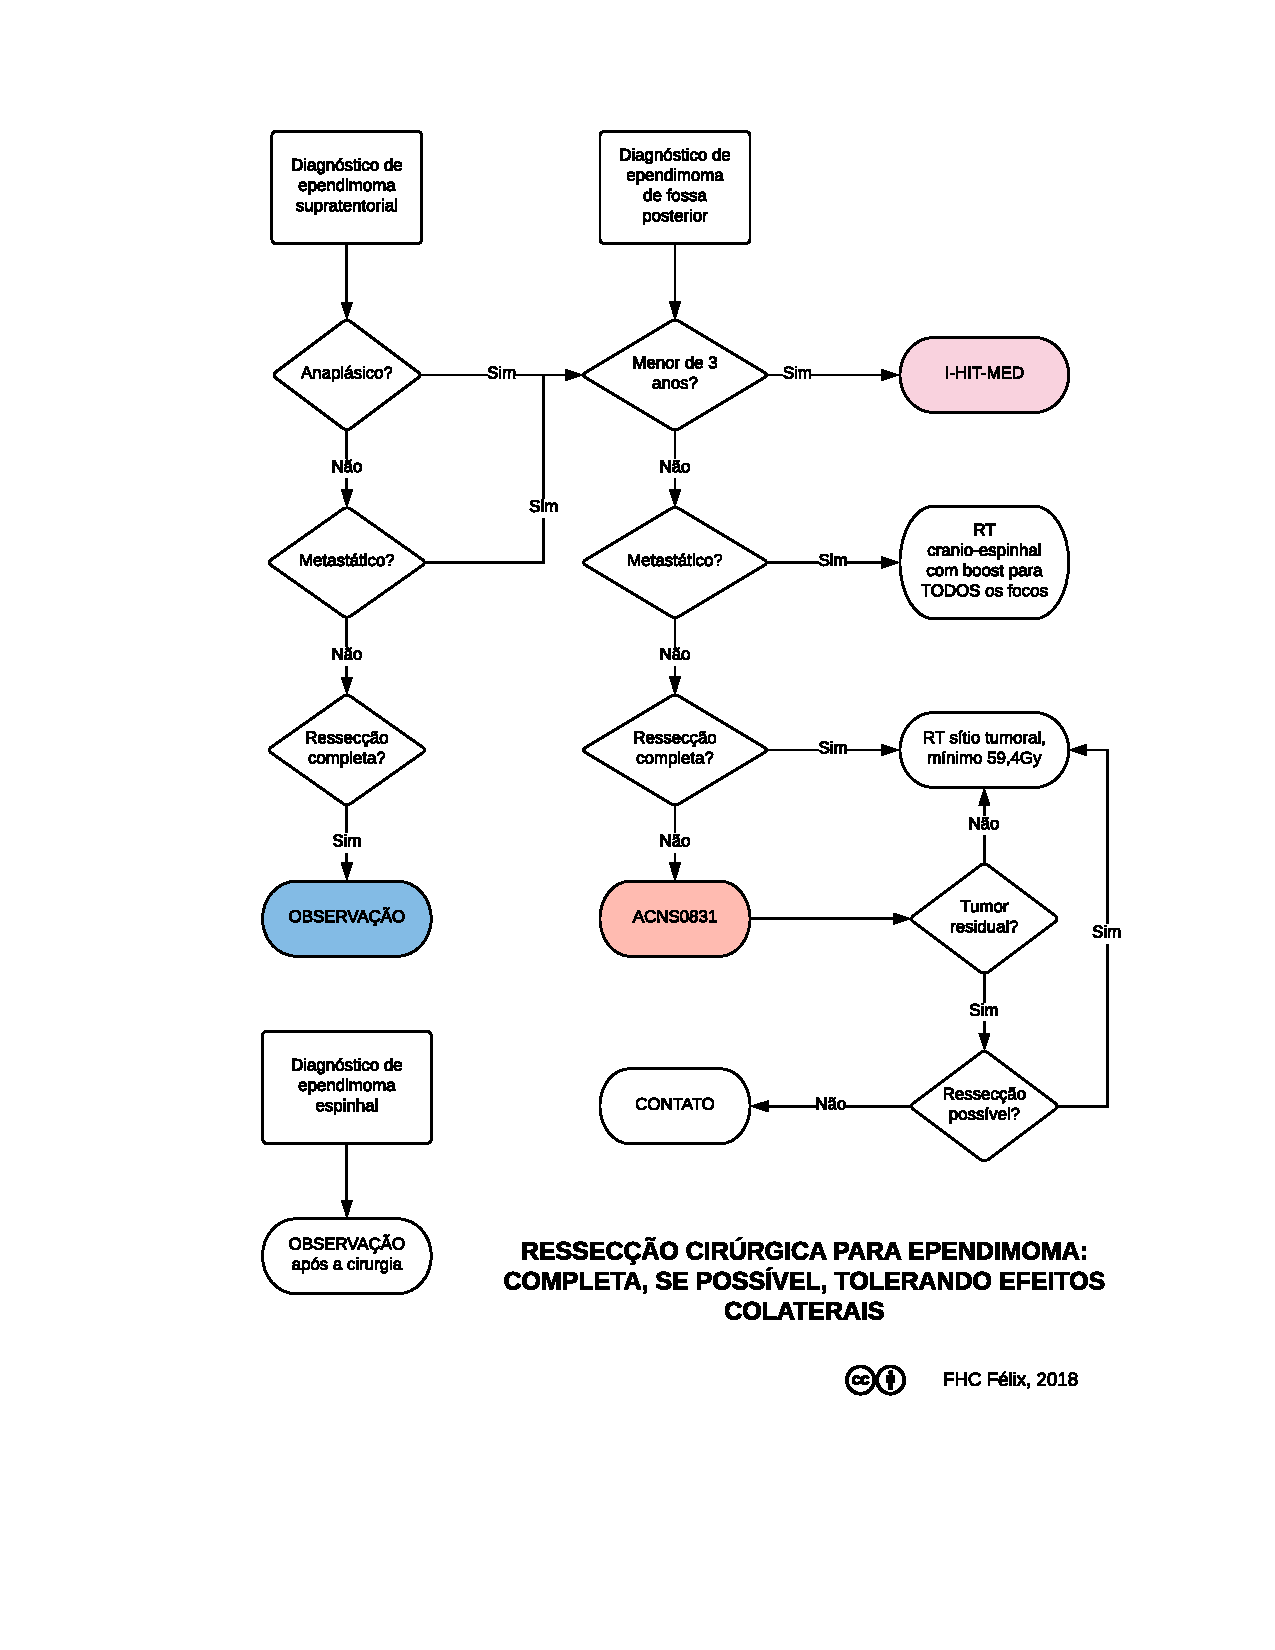
\includegraphics[scale=0.65,trim = 18mm 30mm 15mm 12mm,clip]{fig/fig4.pdf}
\caption{Tratamento de crianças com ependimomas.}
\end{figure}


\begin{figure}[!htb]
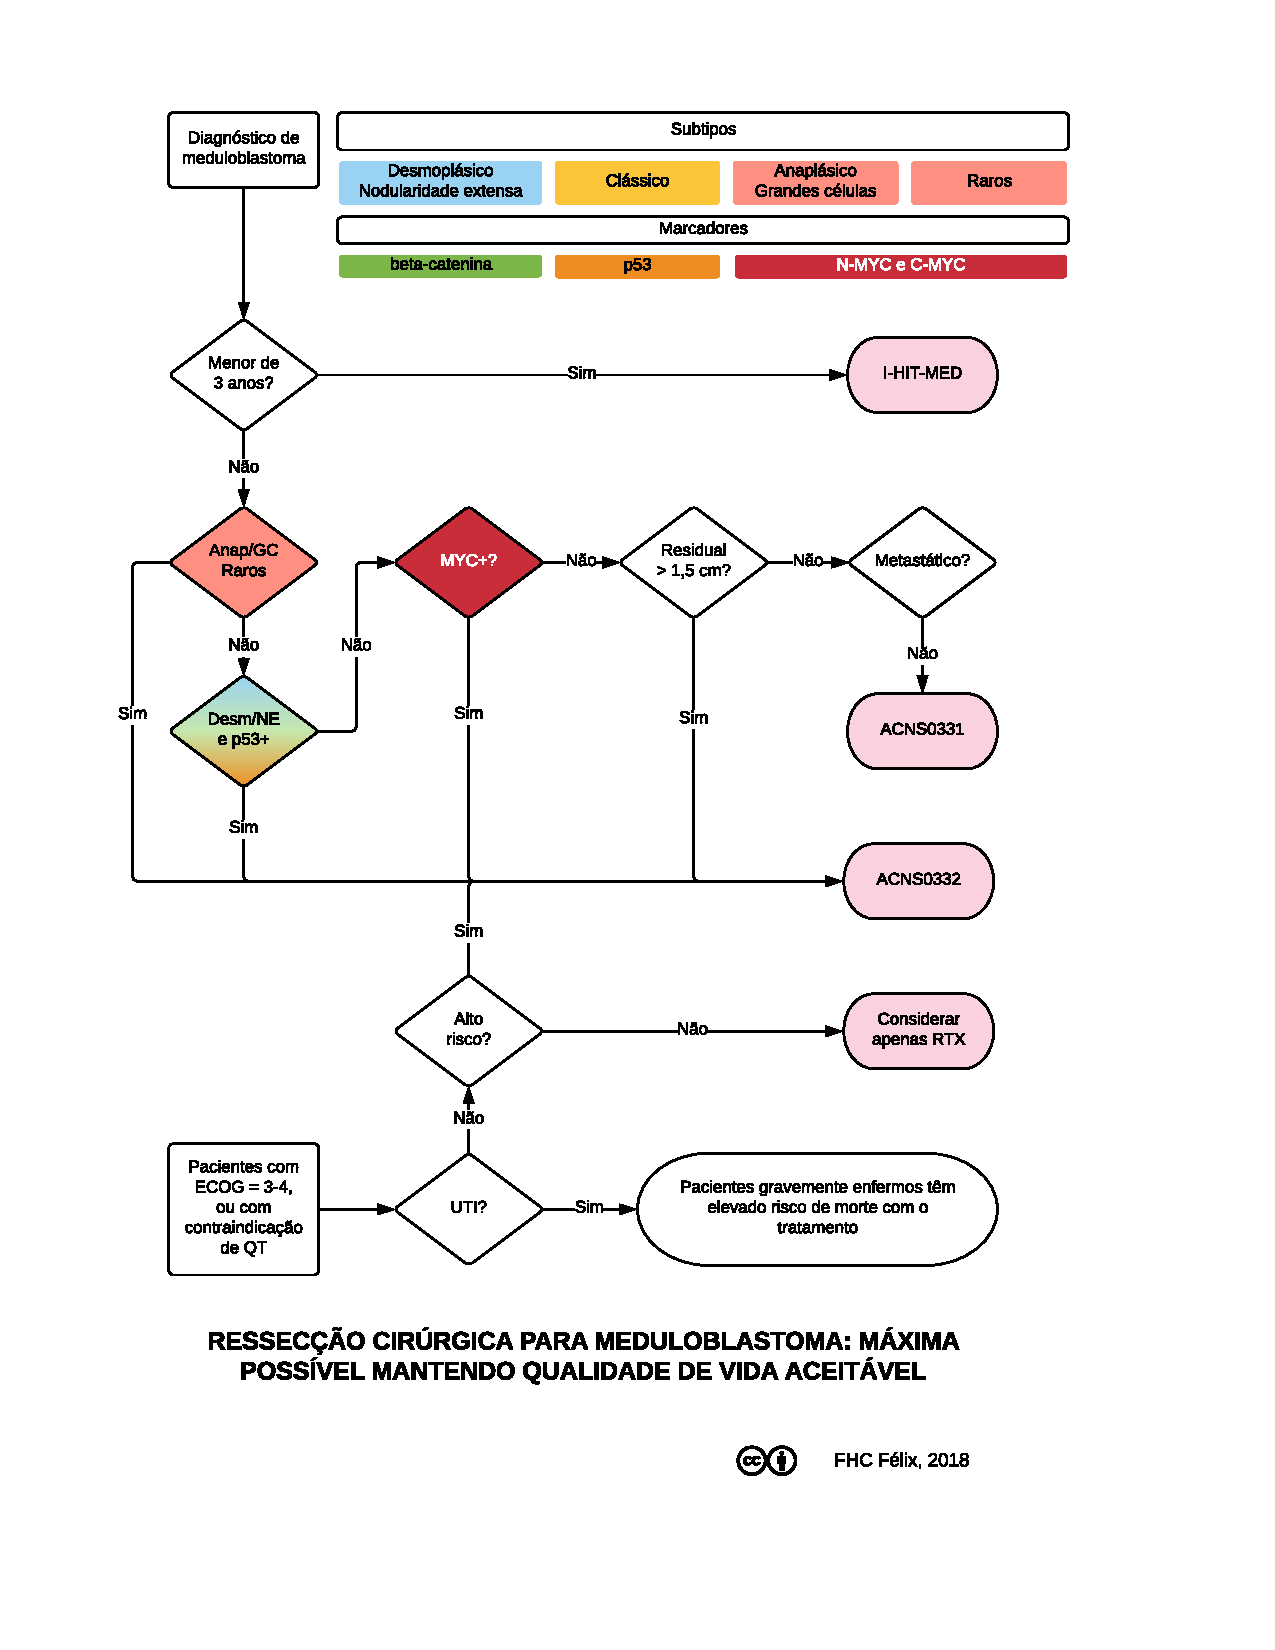
\includegraphics[scale=0.65,trim = 18mm 28mm 15mm 12mm,clip]{fig/fig5.pdf}
\caption{Tratamento de crianças com meduloblastomas.}
\end{figure}

Tumores embrionários incluem o meduloblastoma (mais comum deste grupo e o tumor cerebral maligno mais frequente em crianças e adolescentes), tumor teratóide-rabdóide atípico, tumor embrionário formador de rosetas em multicamadas, tumor embrionário sem outra especificação (SOE) e outros tumores mais raros. 

\begin{center}
\begin{table}
\renewcommand{\arraystretch}{1.5}
	\caption{\tiny }
\begin{tabular}{c|c|c|c|c|c|c}
	\hline
	\multicolumn{1}{c|}{\multirow{11}{*}{Meduloblastoma}}&{\multirow{4}{*}{Desmoplásico/nodular}}&{0-5}&{\multirow{2}{*}{M0}}&{R0+}&{MYC/N(-/+)}&{P1}	\\
	\cline{3-3} \cline{5-7}
	\multicolumn{1}{c|}{}&{}&\multicolumn{1}{c|}{\multirow{3}{*}{>5}}&{}&{R0}&{MYC/N(-/?)}&{P2}
	\\
	\cline{4-7}
	\multicolumn{1}{c|}{}&{}&{}&\multicolumn{1}{c}{M1 ou}&\multicolumn{1}{c}{R+ ou}&{MYC/N(+)}&{P3}
	\\
	\cline{4-7}
	\multicolumn{1}{c|}{}&{}&\multicolumn{1}{c|}{}&{M2/3}&{R0+}&{MYC/N(-/+)}&{P4}
	\\
	\cline{2-7}
	\multicolumn{1}{c|}{}&{\multirow{4}{*}{Clássico}}&{0-3}&{M0}&{R0+}&{MYC/N(-/+)}&{P1}	\\
	\cline{3-7}
	\multicolumn{1}{c|}{}&{}&\multicolumn{1}{c|}{\multirow{3}{*}{>4}}&{M0}&{R0}&{MYC/N(-/?)}&{P2}
	\\
	\cline{4-7}
	\multicolumn{1}{c|}{}&{}&\multicolumn{1}{c|}{}&{M0/1}&{R+}&{MYC/N(+)}&{P3}
	\\
	\cline{4-7}
	\multicolumn{1}{c|}{}&{}&\multicolumn{1}{c|}{}&{M2/3}&{R+}&{MYC/N(-/+)}&{P4}
	\\
	\cline{2-7}
	\multicolumn{1}{c|}{}&{\multirow{3}{*}{Grandes células/anaplásico}}&{0-3}&{M0}&{R0+}&{MYC/N(-/+)}&{P1}	\\
	\cline{3-7}
	\multicolumn{1}{c|}{}&{}&\multicolumn{1}{c|}{\multirow{2}{*}{>4}}&{M0/1}&{R0+}&{MYC/N(-/+)}&{P3}
	\\
	\cline{4-7}
	\multicolumn{1}{c|}{}&{}&\multicolumn{1}{c|}{}&{M2/3}&{R+}&{MYC/N(-/+)}&{P4}
	\\
	\hline
	\multicolumn{2}{c|}{\multirow{3}{*}{Pineoblastoma}}&{0-3}&{M0}&{R0+}&{MYC/N(-/+)}&{P1}	\\
	\cline{3-7}
	\multicolumn{2}{c|}{}&\multicolumn{1}{c|}{\multirow{2}{*}{>4}}&{M0}&{R0+}&{MYC/N(-/+)}&{P3}
	\\
	\cline{4-7}
	\multicolumn{2}{c|}{}&\multicolumn{1}{c|}{}&{M+}&{R+}&{MYC/N(-/+)}&{P4}
	\\
	\hline
	
\end{tabular}
\end{table}
\end{center}


\bibliographystyle{unsrt}
\bibliography{cpc-neuro2014/bib}

\end{document}
